\documentclass{article}
\usepackage[margin=1in]{geometry}
\usepackage{bookmark}
\usepackage{graphicx} % Required for inserting images
\usepackage{float}
\usepackage[titletoc,toc,page]{appendix}
\usepackage{wrapfig}
\usepackage{caption}
\usepackage{subcaption}
\usepackage{mathtools}
\usepackage{authblk}
\usepackage{hyperref}

\usepackage[style=numeric,sorting=none]{biblatex}
\addbibresource{bibliography.bib}

\hypersetup{
    colorlinks,
    citecolor=blue,
    filecolor=blue,
    linkcolor=blue,
    urlcolor=blue
}

\floatstyle{plain} 
\restylefloat{figure}
\title{AST326 Lab 5: Detecting Exoplanet Transits}
\author{Luke Wriglesworth \\ \small luke.wriglesworth@mail.utoronto.ca}
\date{\today}
\begin{document} % Add this line
\maketitle

\begin{abstract}
The exoplanet GJ 1214b is observed during the time of a known transit, and aperture \& differential photometry techniques are applied to 
generate light curves of the host star's flux over time, using a weighted mean reference light curve obtained using the surrounding stars in the images. The reduced light curve of GJ 1214 is plotted, and used to estimate the parameters of GJ 1214b using both a flat-top model, 
as well as a linear least-squares fitting, incorporating limb darkening effects. Over the course of the 54-minute transit, a $1.59\%$ reduction in flux is approximated using the flat-top model, indicating a
planetary radius of around $2.95R_{\oplus}$. The results of the least-squares fitting refine this approximation to $2.93 \pm 0.402 R_{\oplus}$, with
a semi-major axis of $9.746 \pm 1.463 R_{\odot}$, and an orbital inclination of $90.96 \pm 0.297^\circ$. Possible sources of error in these parameters are discussed, and the results are 
discussed in relation to well-known values of these parameters in scientific literature. 


\end{abstract}

\section{Introduction}
Exoplanets are one of the most exciting fields in modern astronomy, as they are the first step in searching for life outside of Earth. 
Exoplanets differ from the planets in our solar system in that they orbit stars other than the Sun. There are many methods that can be used to detect
exoplanets such as Doppler spectroscopy, direct imaging, and astrometry. The method that will be used in this report is called
transit photometry, which utilizes aperture and differential photometry to measure the flux of the host star as the exoplanet passes in front of it.
Not only is this method able to detect exoplanets, but it can also be used to measure properties of the exoplanet like its radius, inclination of orbit, and density.
The exoplanet observed in this report is the super-Earth GJ 1214b, which was first discovered in 2009 by the MEarth Project, using the transit method, the same technique used now. GJ 1214b orbits around the star
GJ 1214, which is a red dwarf star 47.8 light years away from Earth. The observations of GJ 1214 were recorded by the William Herschel Telescope in the Canary Islands, using ACAM, an auxilary 
port camera with a circular field of view. Standard data reduction techniques such as bias subtraction and flat fielding are applied to the images, and aperture and differential photometry are used to measure the flux of GJ 1214 
at the time of the transit. The light curve of GJ 1214 is then plotted, and the parameters of GJ 1214b are estimated using a flat-top model, as well as linear least-squares fitting incorporating limb darkening.

\newpage

\section{Observations \& Data}
In total, 364 30-second exposure images were taken of GJ 1214 the night of May 23, 2011, at the time of a known transit, using the William Herschel Telescope. All of the CCD images are of dimensions $2071\times2148$, with the exception of approximately half of the bias images, which are of dimensions $2501\times2148$. These bias images are discarded, as 
there is sufficient data with the remaining images to perform the necessary noise reduction. The bias and flat-field images are normalized by their exposures times in order to have comparable intensity values, and then median combined
to create a single master flat-field image and bias image. Each of the 364 science images are then bias subtracted and divided by the flat-field image. Due to the circular field of view of ACAM, the images are normalized only 
with respect to the visible region, and the remaining part of the image is removed using a binary mask. An example of a resulting science image is shown in Figure
\ref{fig:science_image}.

\begin{figure}[H]
    \centering
    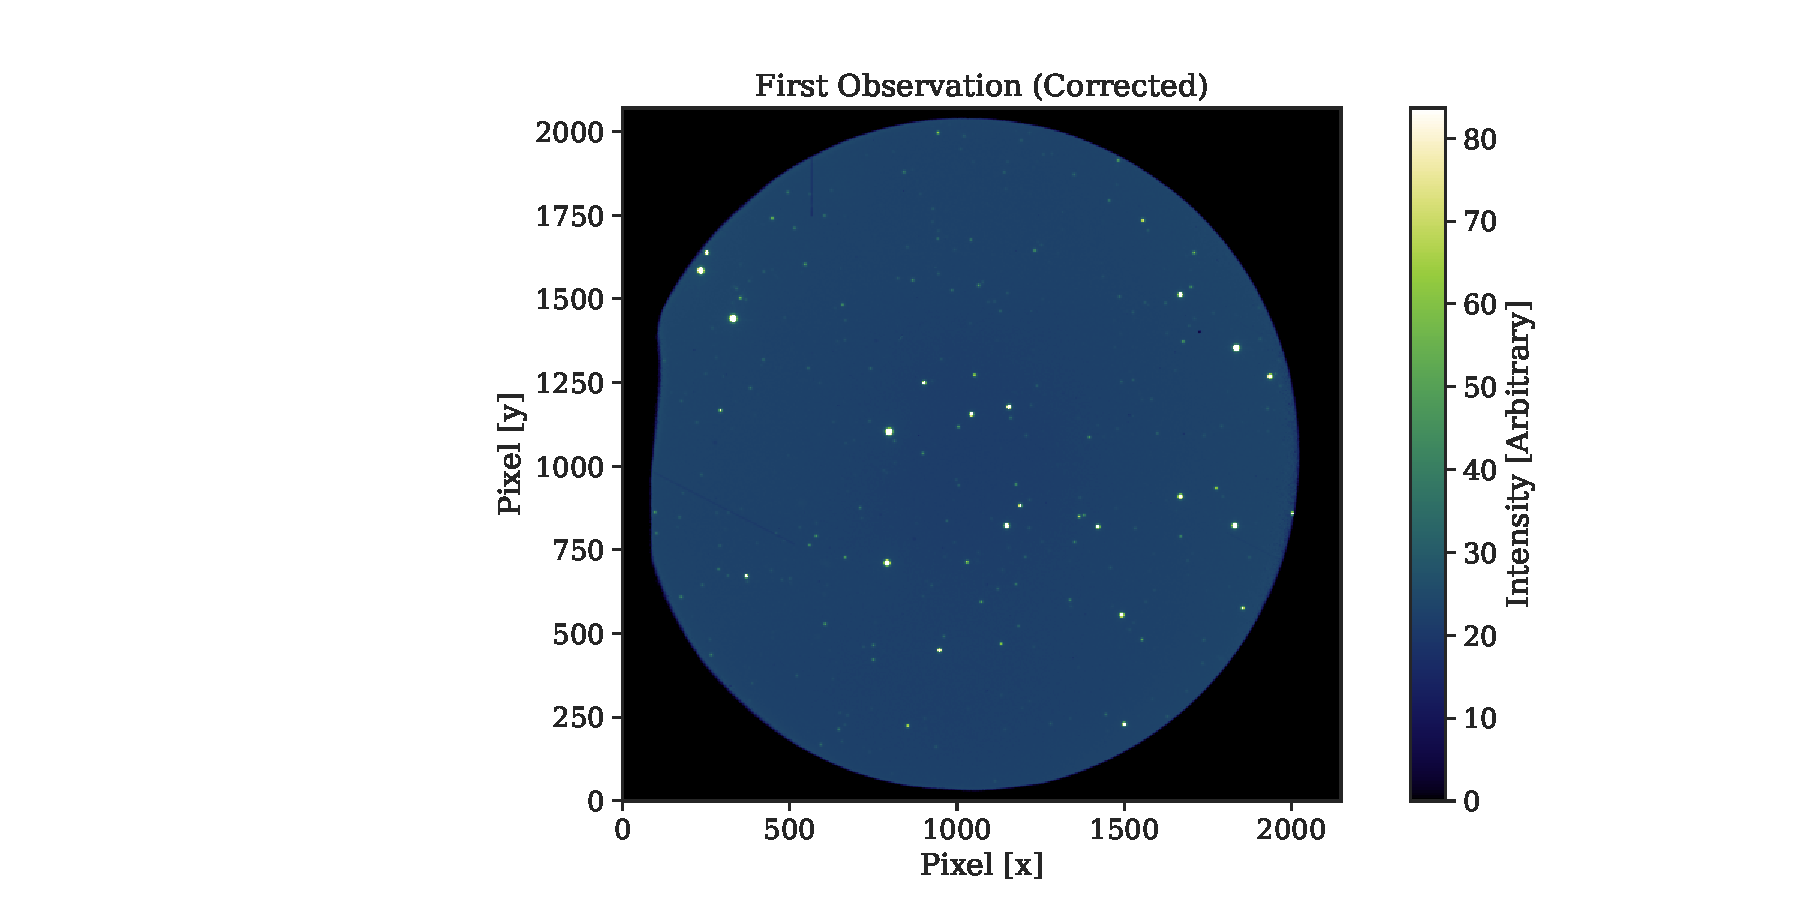
\includegraphics[width=1\textwidth]{plt/science_img.pdf}
    \caption{An example of a corrected science image of GJ 1214, taken with the William Herschel Telescope.}
    \label{fig:science_image}
\end{figure}

\section{Data Reduction \& Methods}
\subsection{Correcting for Star Displacment}
Over the course of the night, the locations of GJ 1214 were tracked by the telescope to some degree. There is significant 
variation observed in the locations of all the stars in the images however. It is also observed that the overall intensity of the images is not constant. This is 
likely due to the changing atmospheric conditions over course of the night, influencing the overall visibility. While the intensity changes can be 
negated using aperture photometry, the changing positions of the stars in the images is a more complicated task. To solve this issue without recomputing 
each of the stars centroids in every frame, a single star is instead chosen as a reference, approximating the relative changes in position of all the stars at once. 
Even though this method is not perfect, it is observed that it reduced the motion of the centroids down to a 1-2 pixel range in each image, so it is deemed to be sufficient for 
the purposes of this report. The tracked pixel displacements in $x$ and $y$, as well as displacement magnitude of the chosen reference star are shown in Figure \ref{fig:ref_star} 

\begin{figure}[H]
    \centering
    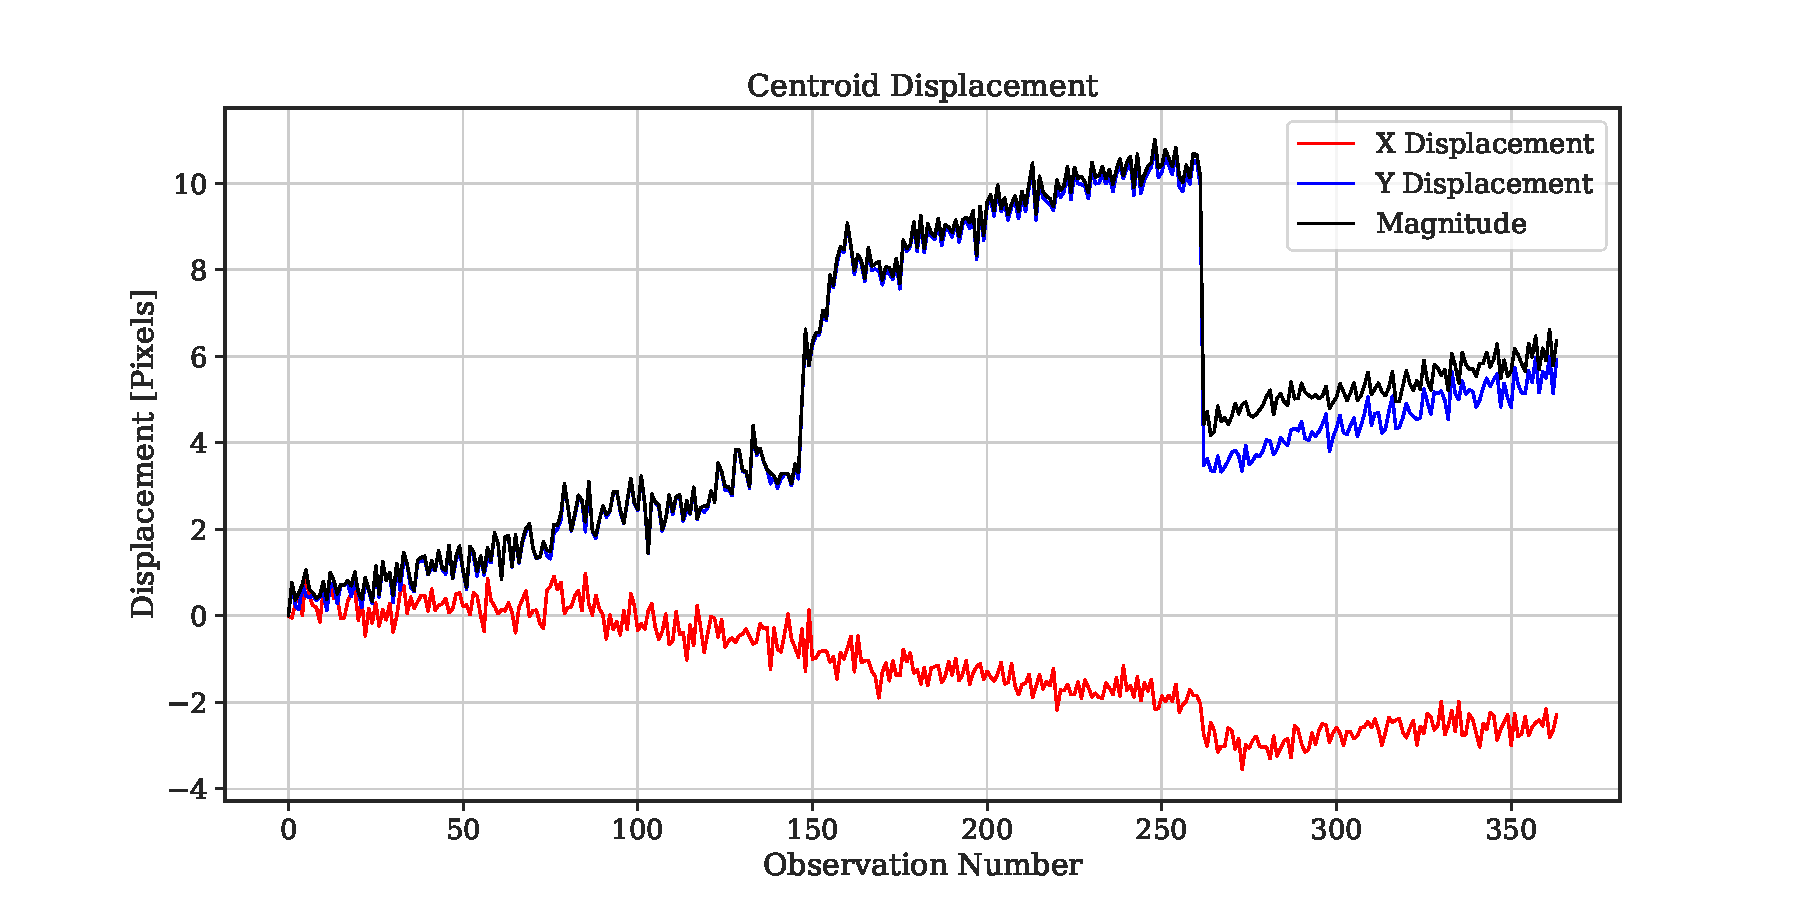
\includegraphics[width=1\textwidth]{plt/centroid_displacement.pdf}
    \caption{The tracked pixel displacement in $x$ and $y$, as well as displacement magnitude of the chosen reference star.}
    \label{fig:ref_star}
\end{figure}

\subsection{Reference Star Selection and Centroiding}
The most prominent reference stars are now selected in the images, and the approximate pixel positions are measured
using a binary mask intensity threshold. Special care is taken to avoid any images that move out of the field of view of 
ACAM over the course of the night by selecting only stars that are present in all the images, and avoiding stars near any dead pixels. 
The selected reference stars are shown in Figure \ref{fig:ref_stars}. Although GJ 1214 is shown as a selected star in this figure, it 
was manually removed prior to creating the light curves for differential photometry. 

\begin{figure}[H]
    \centering
    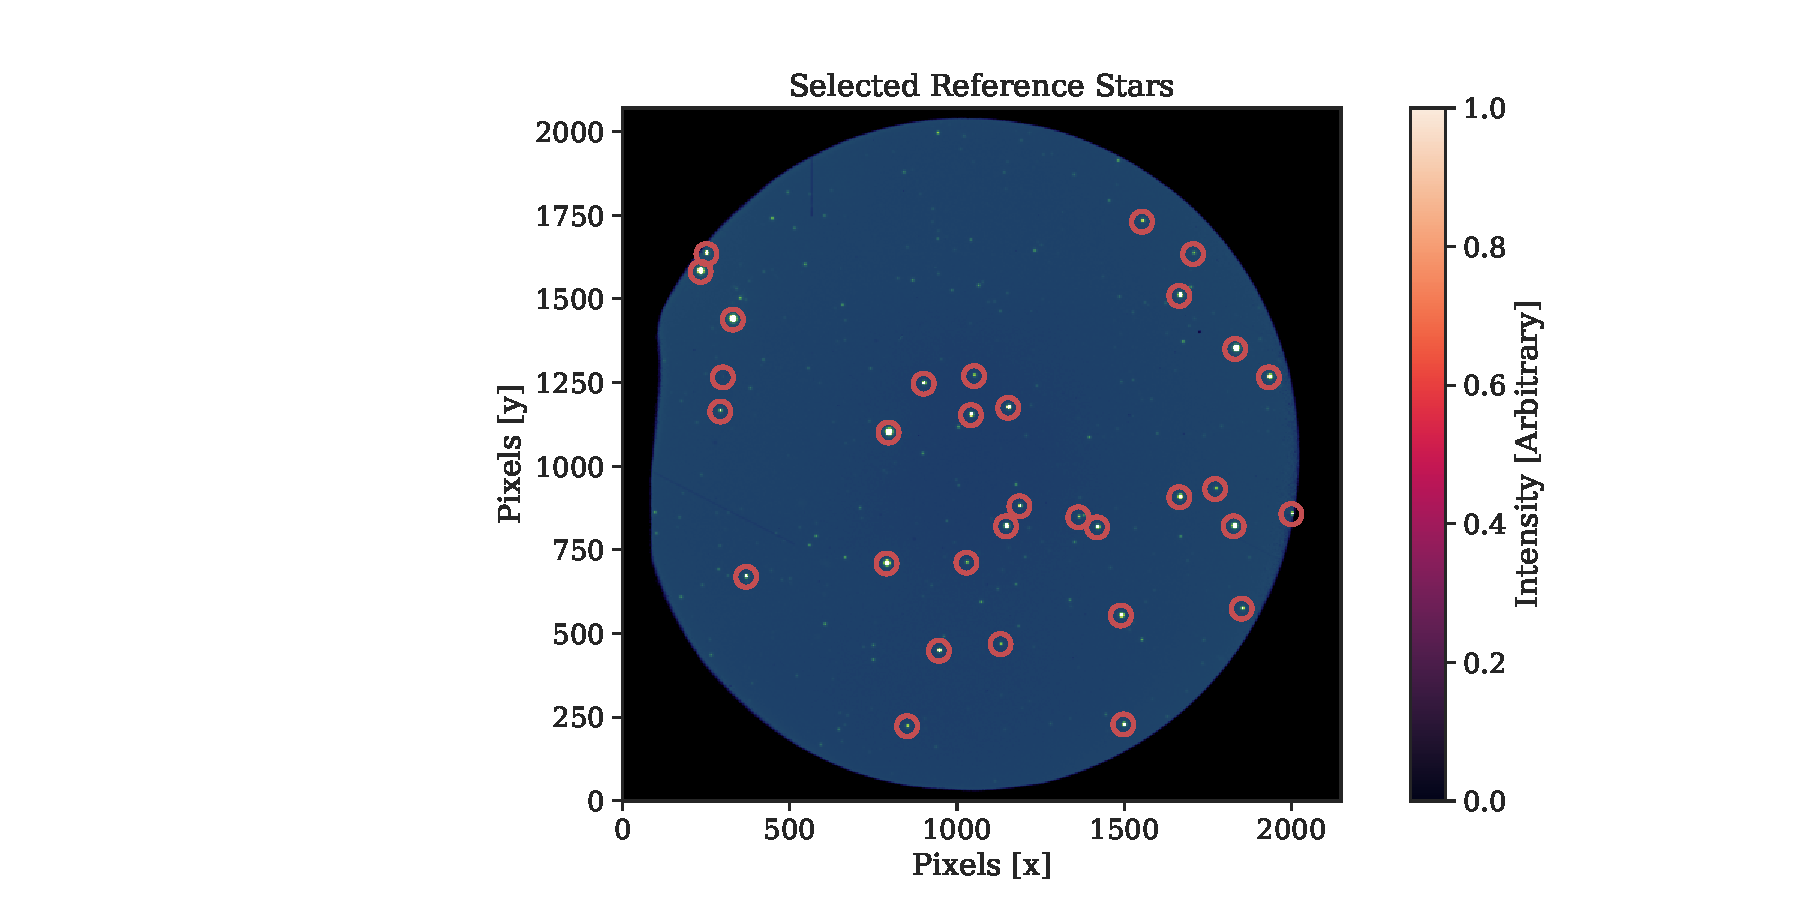
\includegraphics[width=1\textwidth]{plt/selected_reference_stars.pdf}
    \caption{The selected reference stars in the images.}
    \label{fig:ref_stars}
\end{figure}

To further improve these position estimations, the centroids of the reference stars are measured using both the traditional centroid method, as well 
as a two-dimensional Gaussian fit. The Gaussian fitting not only improves the initial position estimations, but also provides a convenient way of calculating uncertainties 
in the position measurements, as well as computing appropriate aperture radii. 3-times the standard deviation of each star's Gaussian function was chosen to be the radius for each of the star's aperture's when performing 
aperture photometry. The results of this fitting process are shown in figure \ref{fig:centroid_fit}.

\begin{figure}[H]
    \centering
    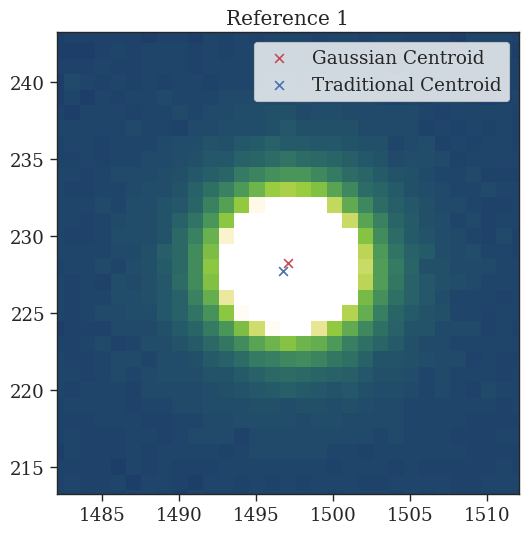
\includegraphics[width=.4\textwidth]{plt/gauss_cent.png}
    \caption{The results of the centroid fitting process.}
    \label{fig:centroid_fit}
\end{figure}

After examining each of the centroids of the reference stars throughout the night and confirming that the centroid tracking method is working as expected, aperture photometry is now almost ready to be 
performed. Despite the attempts to avoid any dead pixel regions, it is observed that some of these questionable stars were missed when selecting them earlier, and discarded from the analysis. An example of one of these
discarded stars is shown in Figure \ref{fig:discarded_star} located near the edge of ACAM's field of view. It is difficult to tell from looking at the entire image, but the star is close enough to the edge
of the field of view, such that the background noise level is unable to be determined with any precision. 

\begin{figure}[H]
    \centering
    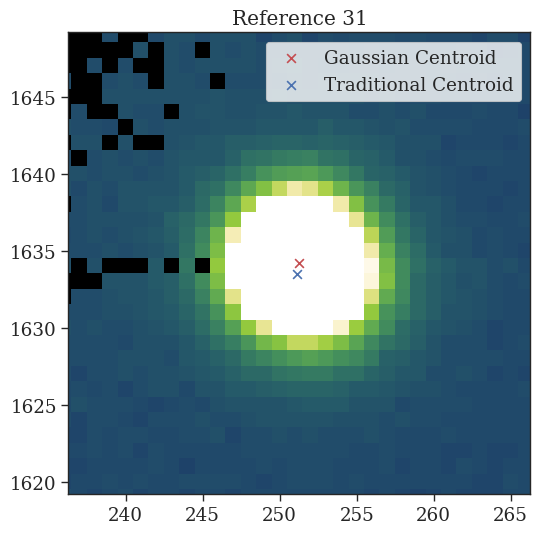
\includegraphics[width=.4\textwidth]{plt/discard.png}
    \caption{An example of a star that has background noise levels that are unable to be determined.}
    \label{fig:discarded_star}
\end{figure}

\subsection{Aperture Photometry}

Aperture photometry is now performed on each of the chosen reference stars, as well as GJ 1214. The aperture radius is chosen to be 3 times the standard deviation 
of the Gaussian fitting of the star's point spread function in the first image. By dynamically adjusting the aperture size in this way, all of the star's light 
can be captured, while also allowing the results of the measurements to be comparable to each other, since each stars aperture is determined in the same way based on its size. An example
of an aperture and annulus measurement being applied to GJ 1214 are shown in Figure \ref{fig:aperture}.


\begin{figure}[H]
    \centering
    \begin{subfigure}{.5\textwidth}
        \centering
        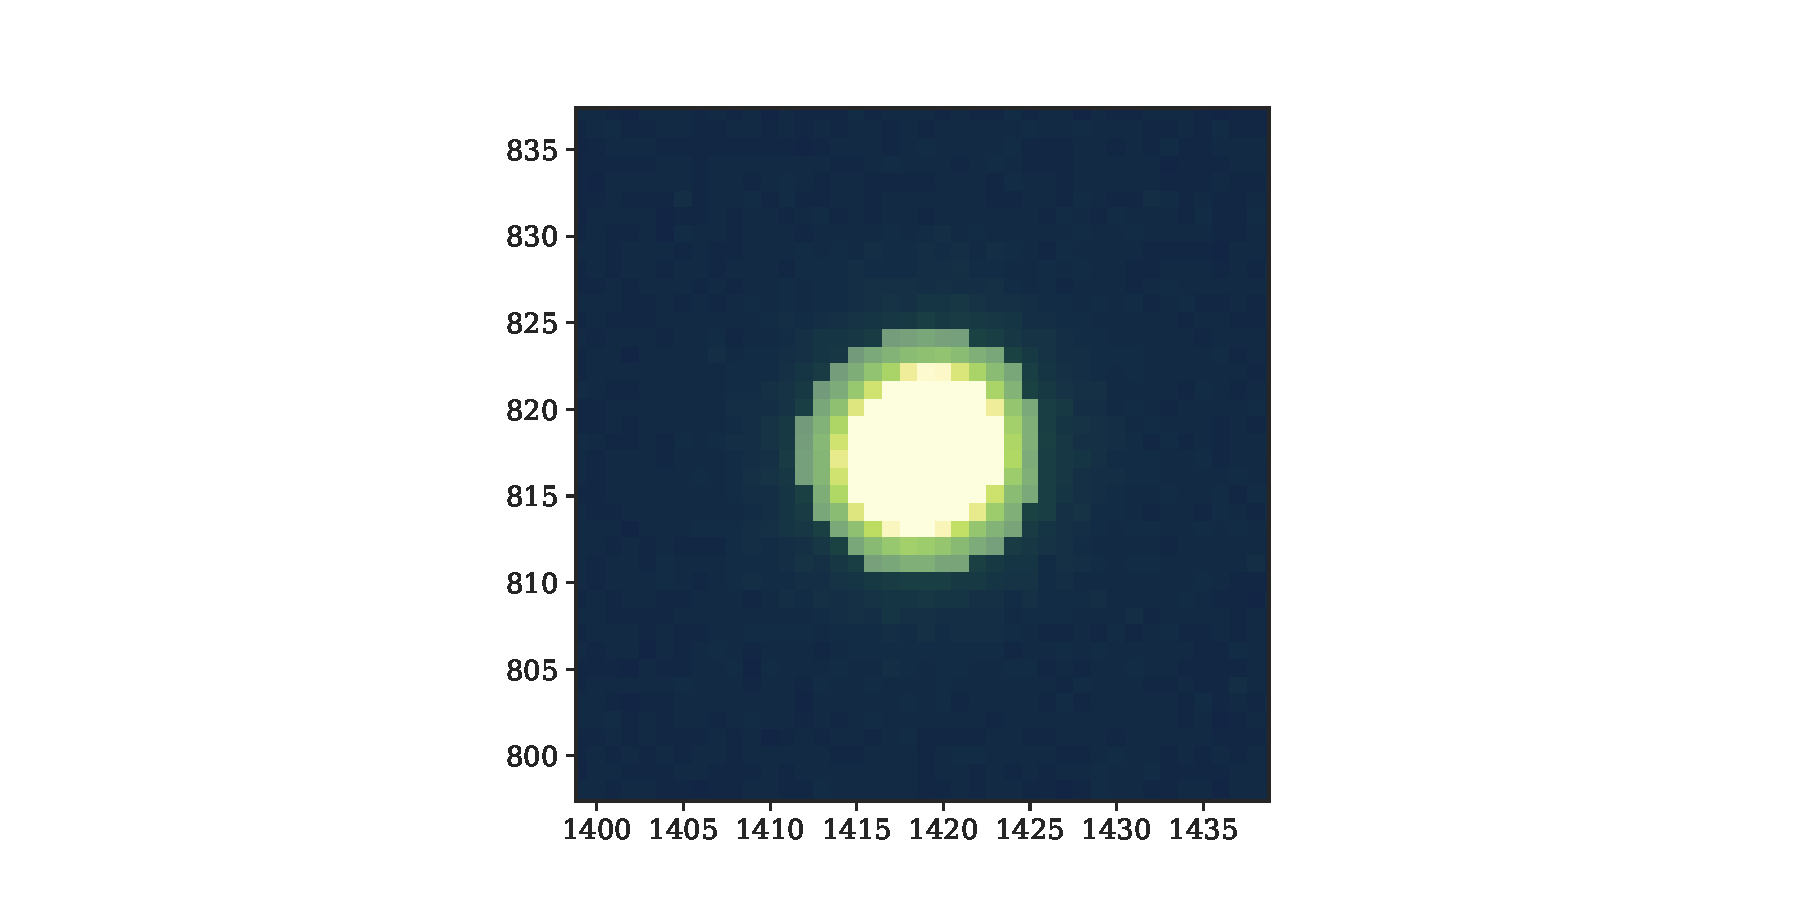
\includegraphics[width=\linewidth]{plt/aperture.pdf}
        \caption{Aperture Measurement of GJ 1214}
        \label{fig:app}
    \end{subfigure}%
    \begin{subfigure}{.5\textwidth}
        \centering
        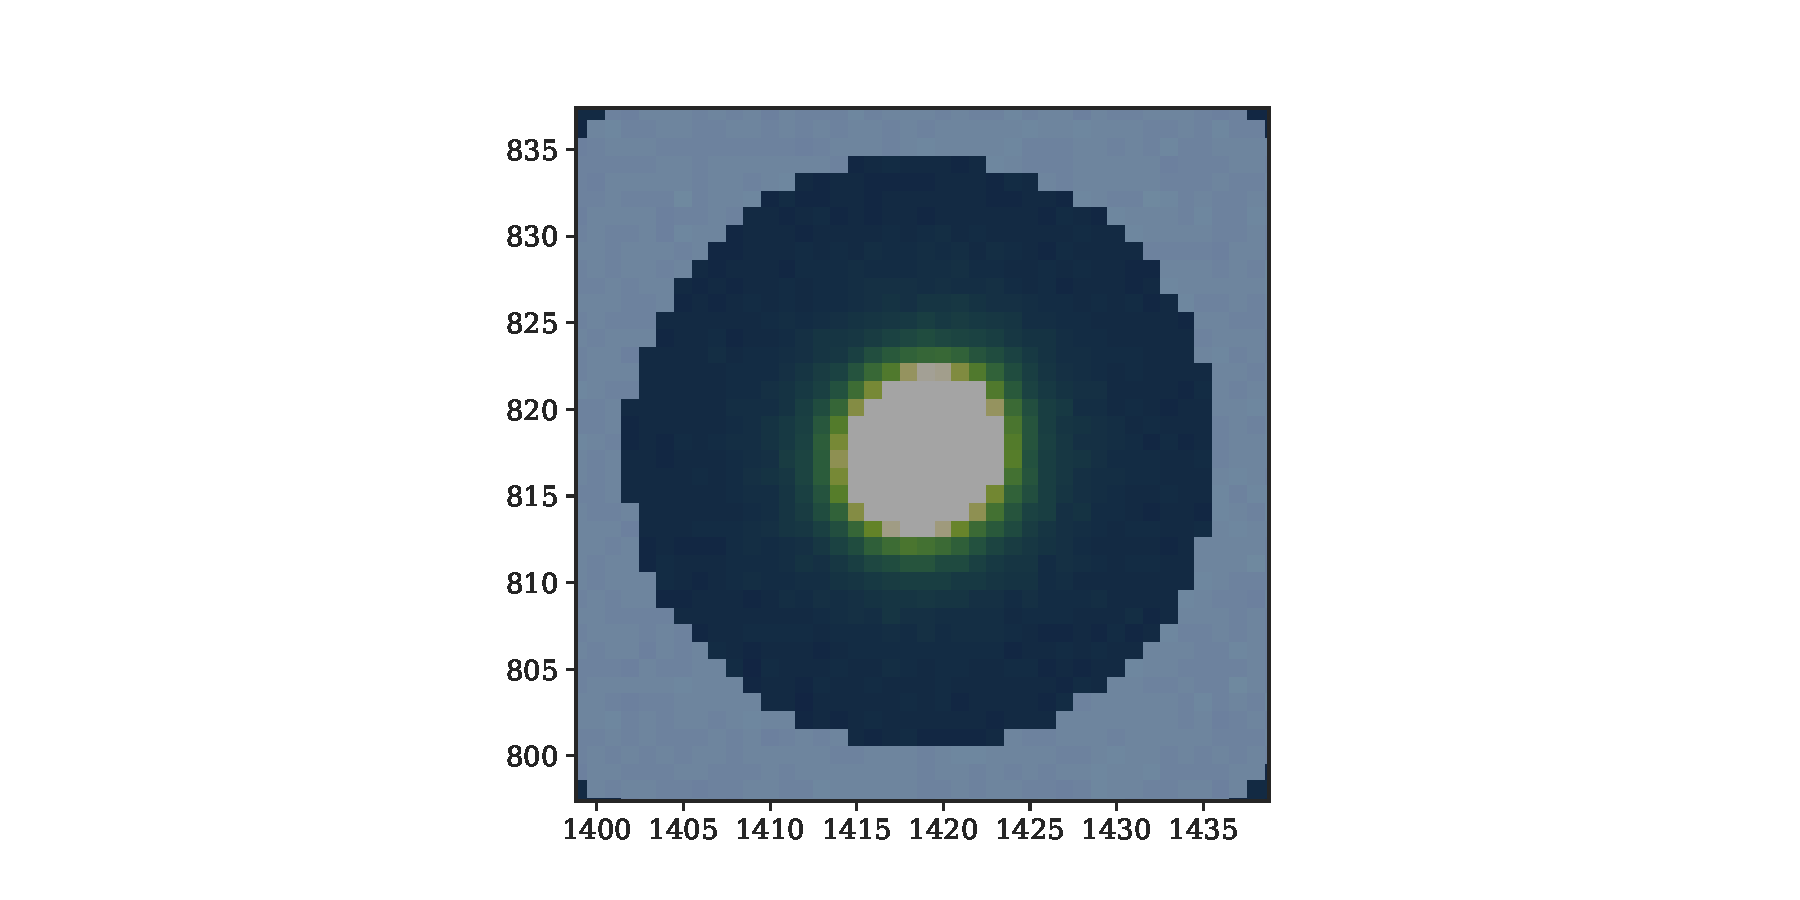
\includegraphics[width=\linewidth]{plt/annulus.pdf}
        \caption{Annulus Measurement of GJ 1214}
        \label{fig:ann}
    \end{subfigure}
    \caption{Aperture and Annulus Measurements of GJ 1214.}
    \label{fig:aperture}
\end{figure}

The width of the annulus is chosen arbitrarily, with its inner radius determined by the radius of the aperture. A translation is applied to the aperture and annulus according to the displacement vector generated by the reference star tracking. The normalized flux 
of GJ 1214 is shown in Figure \ref{fig:target_flux}. To compute the error in flux measurements, a gain of 4 electrons per ADU is assumed based on the lab manual, and the following flux uncertainty formula is utilized \cite{flux_uncertainty}:

\begin{gather}
\delta F = \sqrt{\frac{F}{g} + N_{aperture}(1+\frac{\pi}{2}\frac{N_{aperture}}{N_{annulus}})\sigma_{bg}^2}
\end{gather}

\begin{figure}[H]
    \centering
    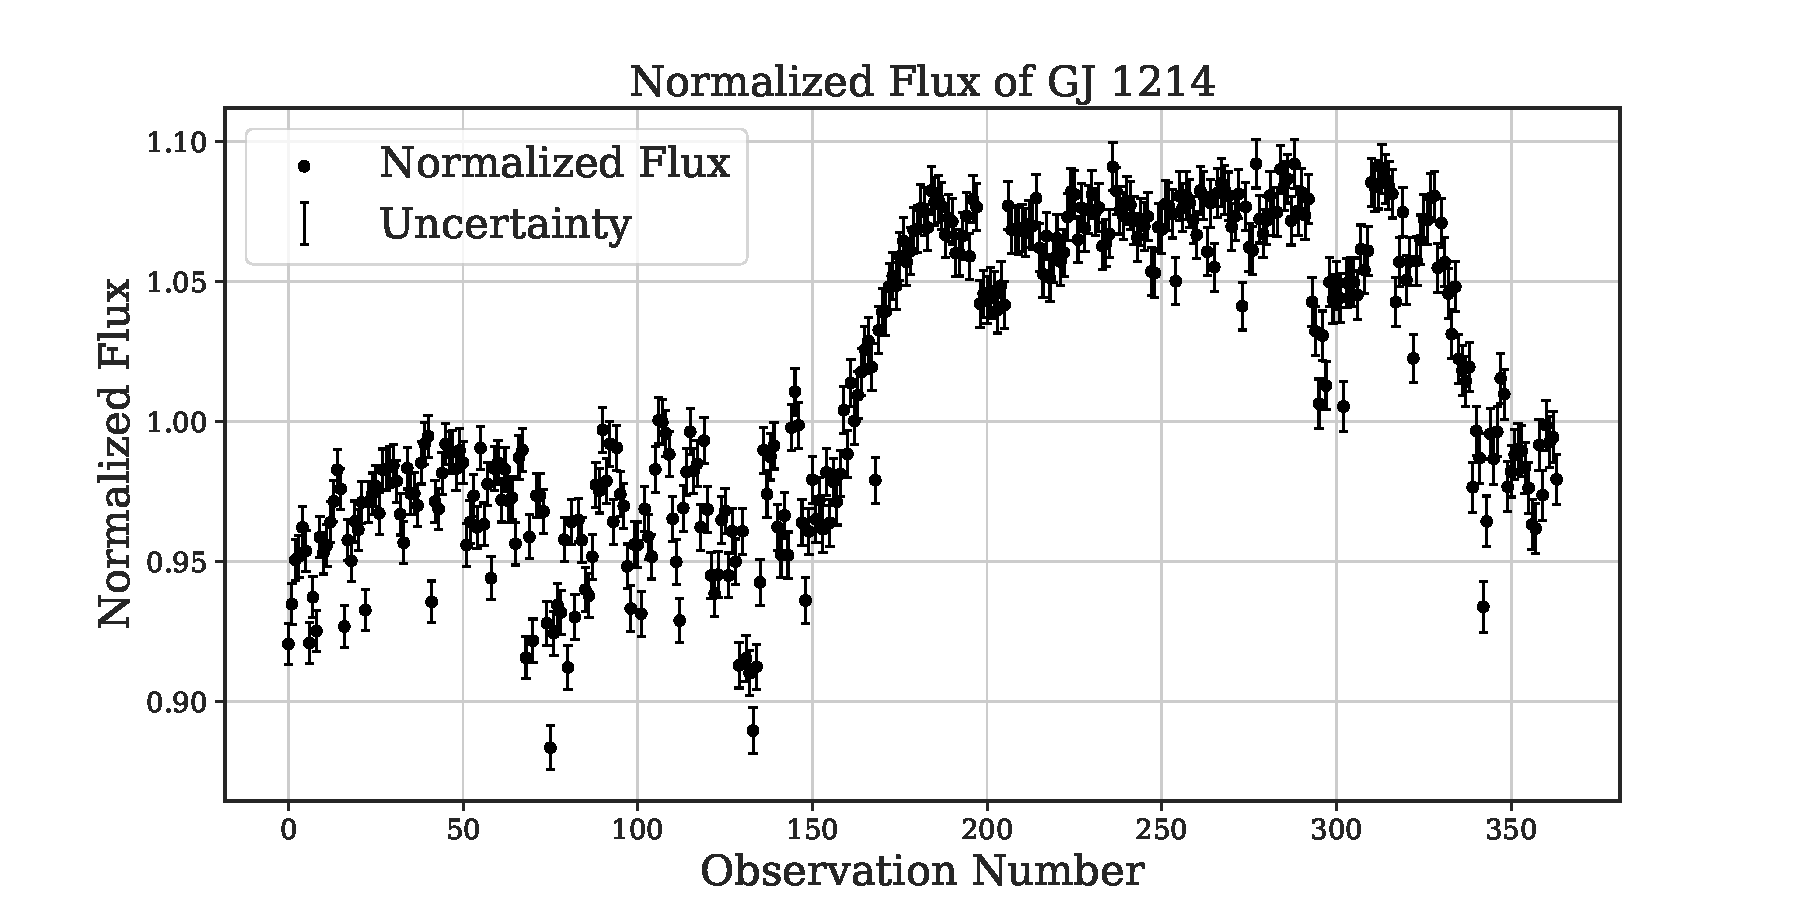
\includegraphics[width=1\textwidth]{plt/target_light_curve.pdf}
    \caption{The normalized flux of GJ 1214, plotted with respect to observation number.}
    \label{fig:target_flux}
\end{figure}


\subsection{Light Curve Analysis}
After running the aperture photometry routine on all of the reference stars and normalizing their curves to unity, it is observed that most of the light curves follow 
a similar pattern, with GJ 1214 included. An example of the raw measurements taken of the first 15 reference stars are shown in Figure \ref{fig:raw_light_curves}.

\begin{figure}[H]
    \centering
    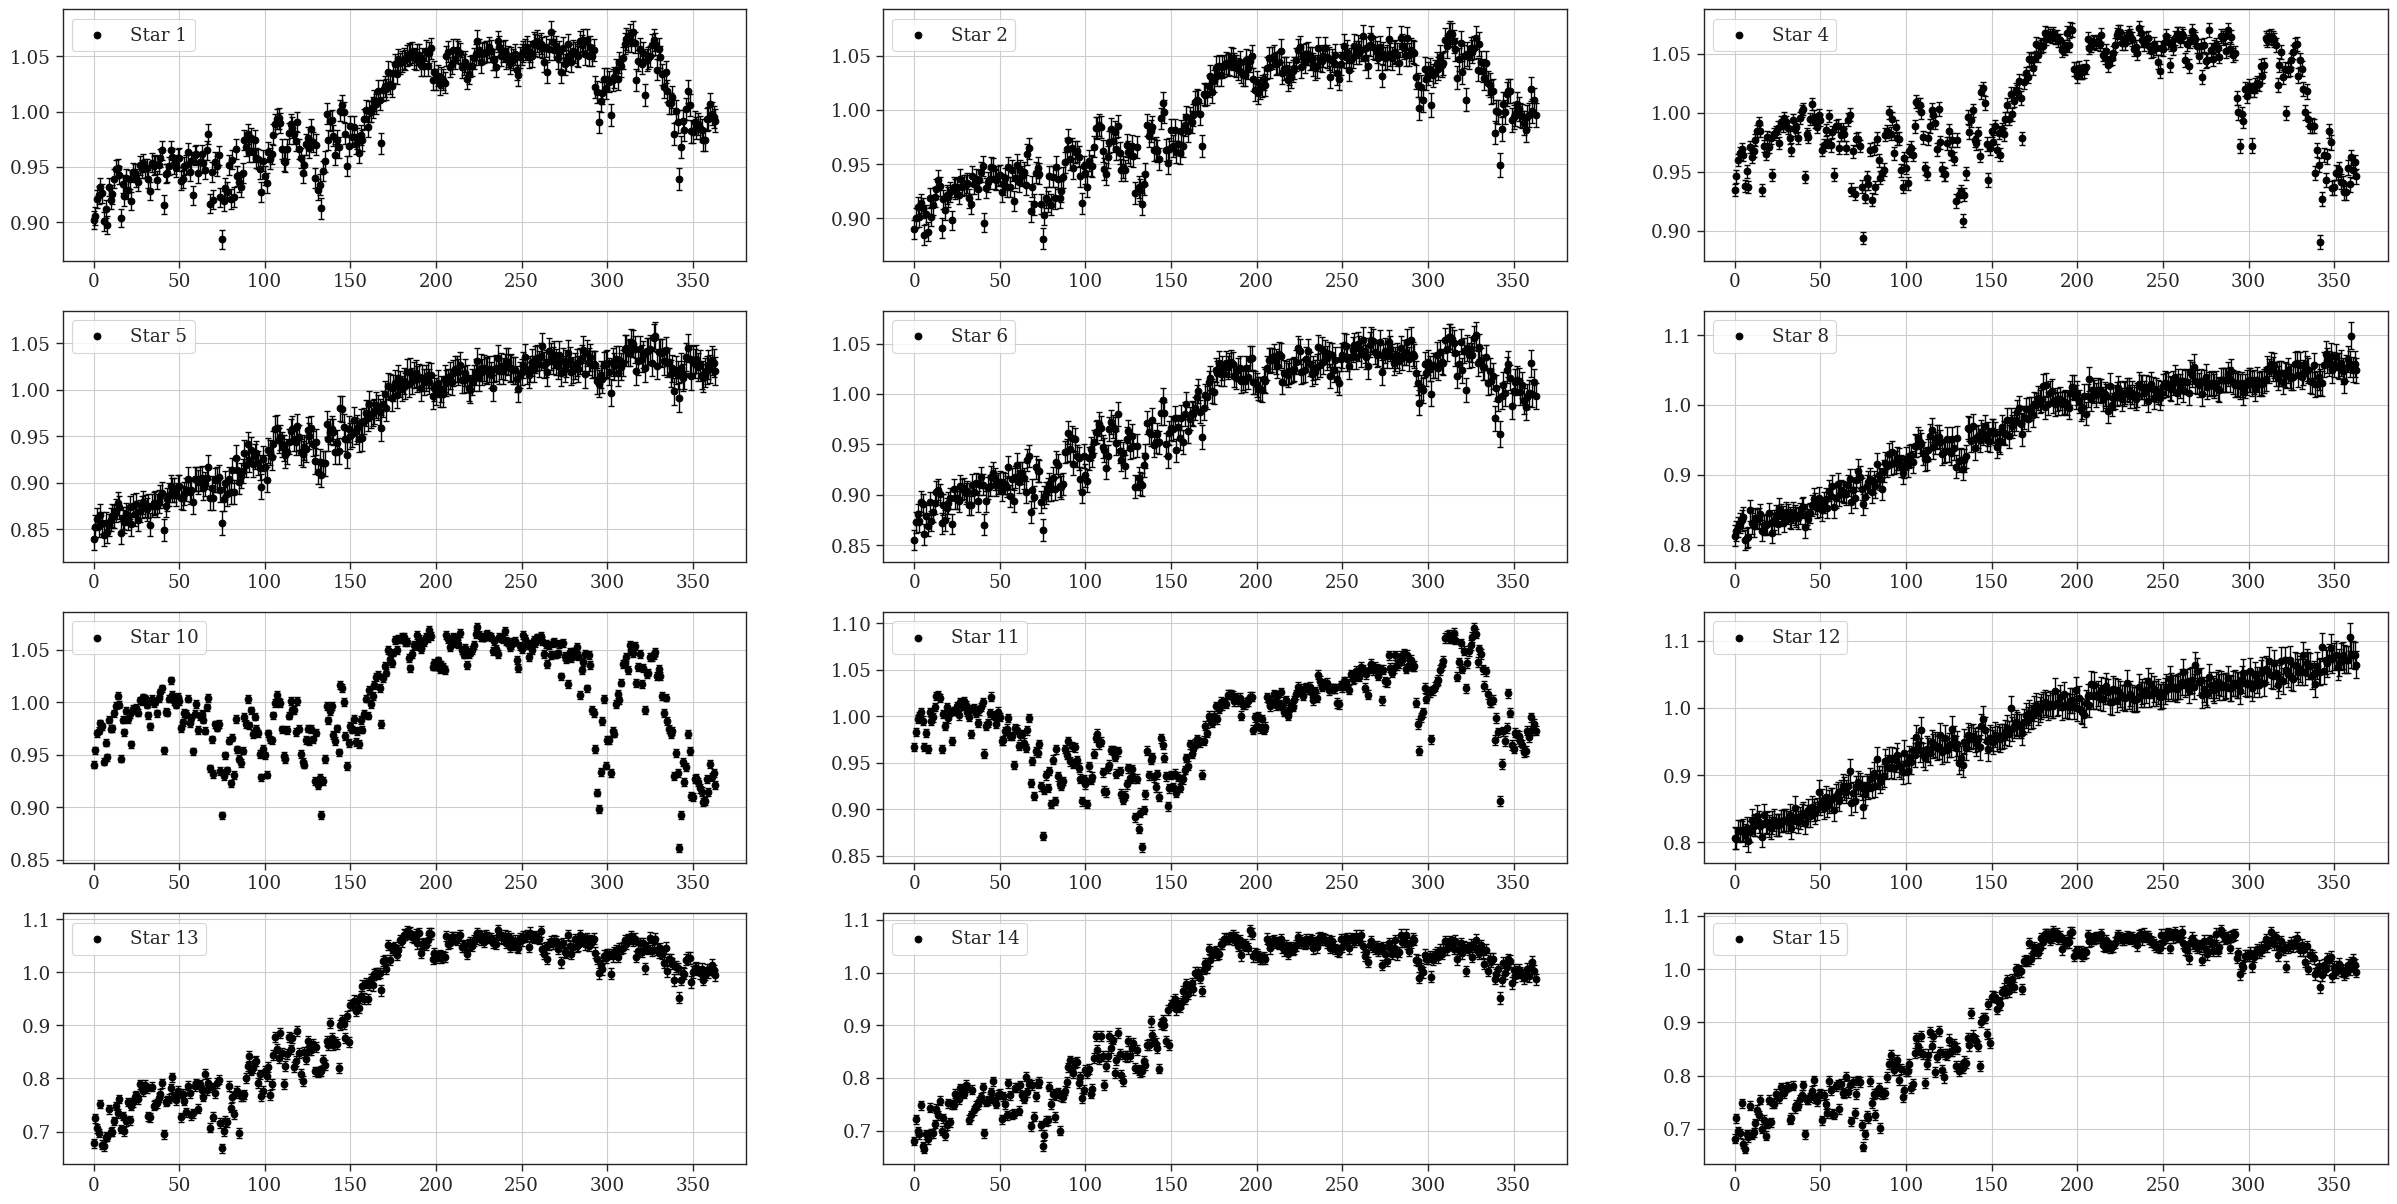
\includegraphics[width=1\textwidth]{plt/curves.png}
    \caption{The normalized flux measurements and their uncertainties taken of the first 15 reference stars, plotted with respect to observation number.}
    \label{fig:raw_light_curves}
\end{figure}

Given that we are only interested in performing differential photometry on GJ 1214, the light curves most closely resembling the overall trend observed in GJ 1214's light curve are 
prioritized as being the most promising. These light curves will contain the same shared atmospheric variations and noise that we are attempting to remove using differential photometry.
In the measurements shown in Figure \ref{fig:raw_light_curves}, it is observed that around 7 of these light curves demonstrate such a trend, with the same 
overall shape and rise in flux between observations 150 and 200. Not all of the light curves differing from this trend are thrown out, however the curves that look nothing like the curve of GJ 1214b are.

\subsection{Master Light Curve Generation \& Differential Photometry}
With the selected light curves in hand, we are now ready to perform differential photometry on GJ 1214 to generate its true light curve, removing the broad changes in flux seen in all the stars in the image.
To generate the master light curve for differential photometry, two methods are attempted. The first method is to simply take the median of the selected light curves. The results of this method are shown in Figure 
\ref{fig:median_master}. 

\begin{figure}[H]
    \centering
    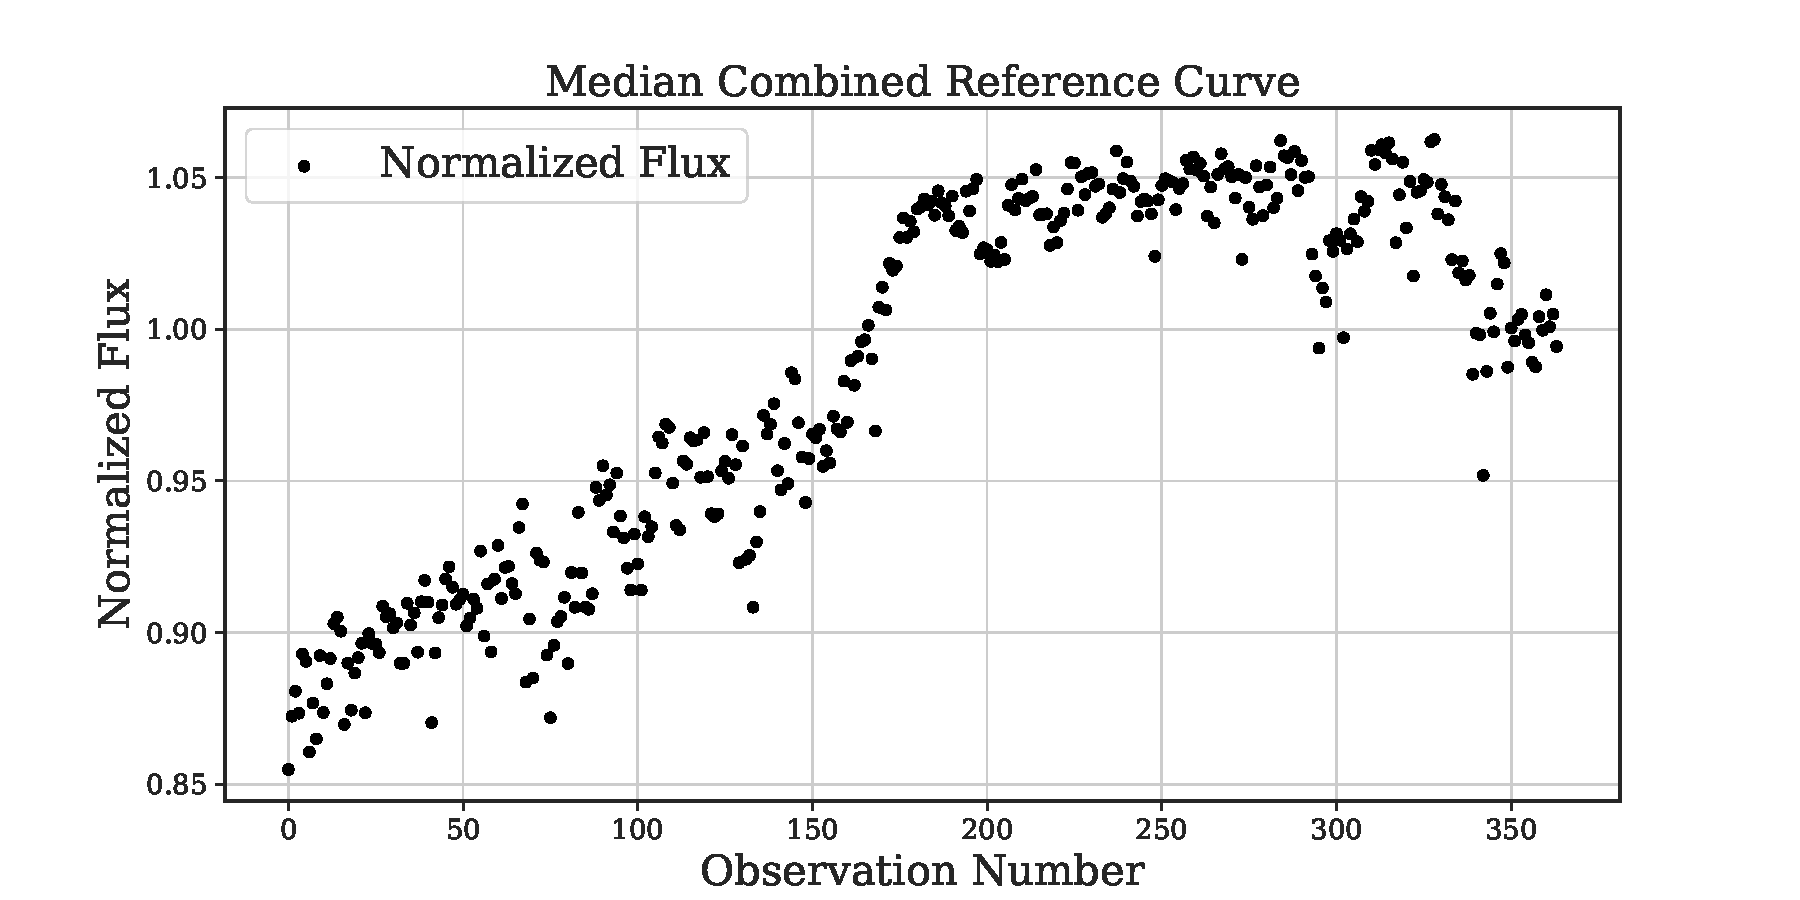
\includegraphics[width=.75\textwidth]{plt/median_reference_curve.pdf}
    \caption{The master light curve generated by taking the median of the selected light curves.}
    \label{fig:median_master}
\end{figure}

While the median combination method shown in Figure \ref{fig:median_master} looks very promising visually, it did not perform very well when dividing GJ 1214's light curve by it. Furthermore, we also 
have uncertainties in the flux measurements of the reference stars, so it makes much more sense to make use of those and perform a weighted mean combination. This method 
provides a master light curve minimizing the uncertainties in the flux measurements. The results of this method are shown in Figure \ref{fig:mean_curve}.

\begin{figure}[H]
    \centering
    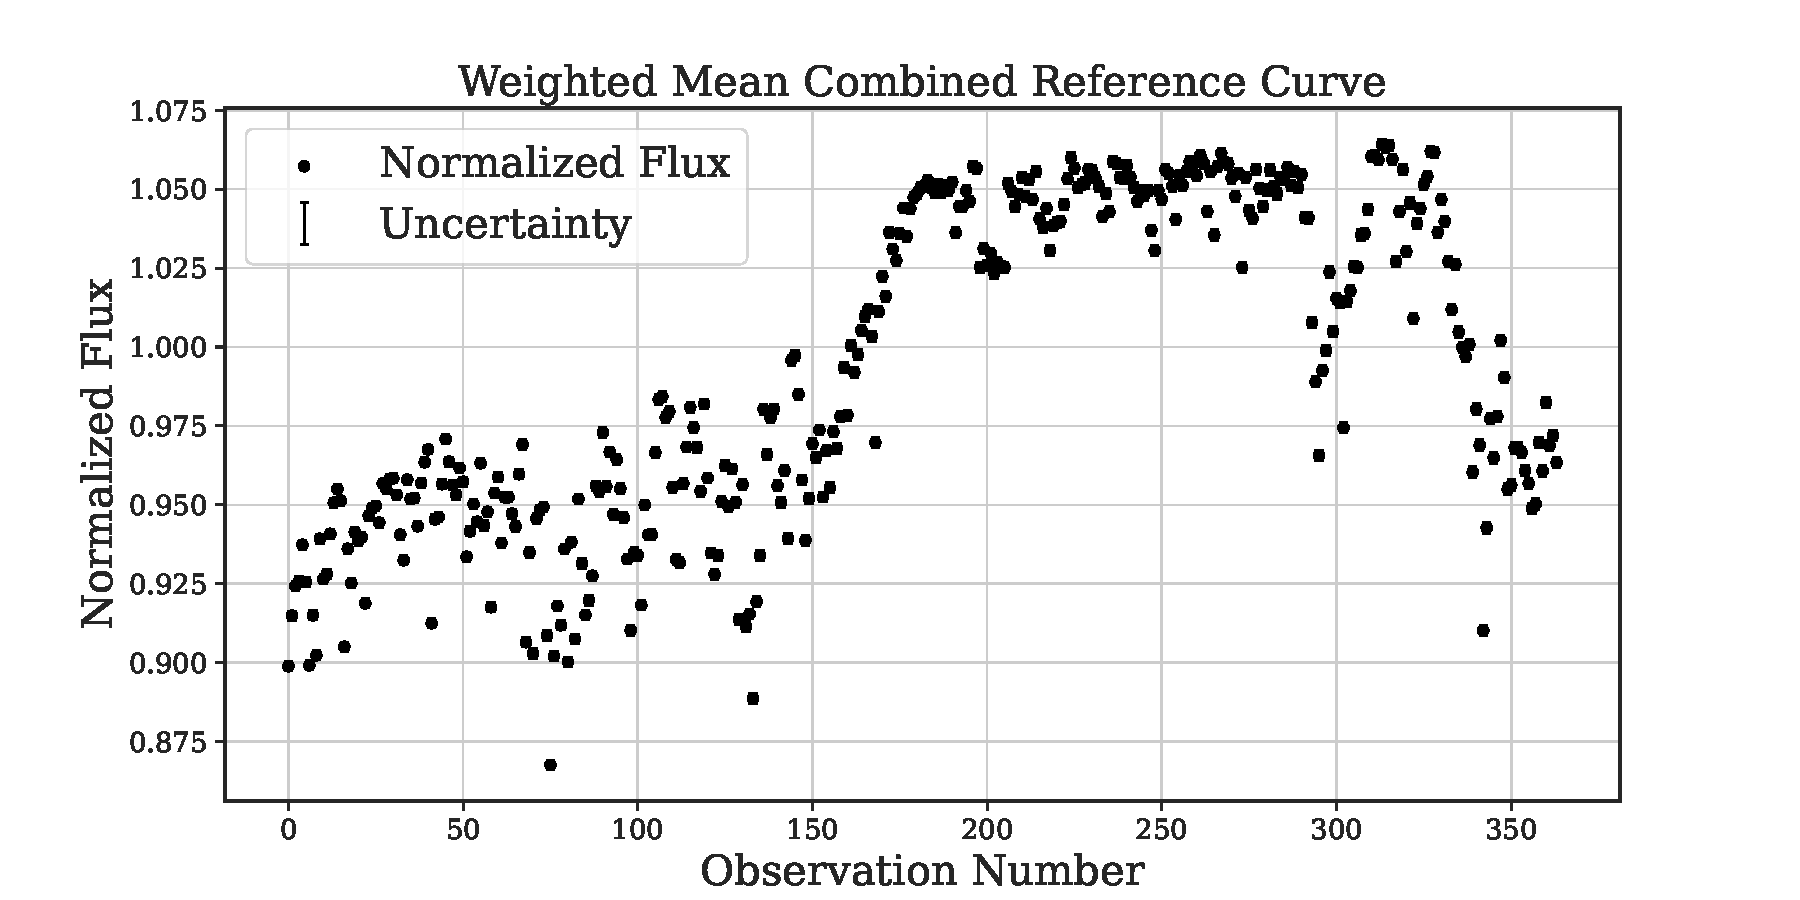
\includegraphics[width=.75\textwidth]{plt/weighted_mean_reference_curve.pdf}
    \caption{The master light curve generated by taking the weighted mean of the selected light curves.}
    \label{fig:mean_curve}
\end{figure}

The normalized flux of GJ 1214 is then divided by the master light curve generated by the weighted average. The reduced light curve
during the time of GJ 1214b's transit is shown in Figure \ref{fig:reduced_curve}, from the observations between 0 and 300.

\begin{figure}[H]
    \centering
    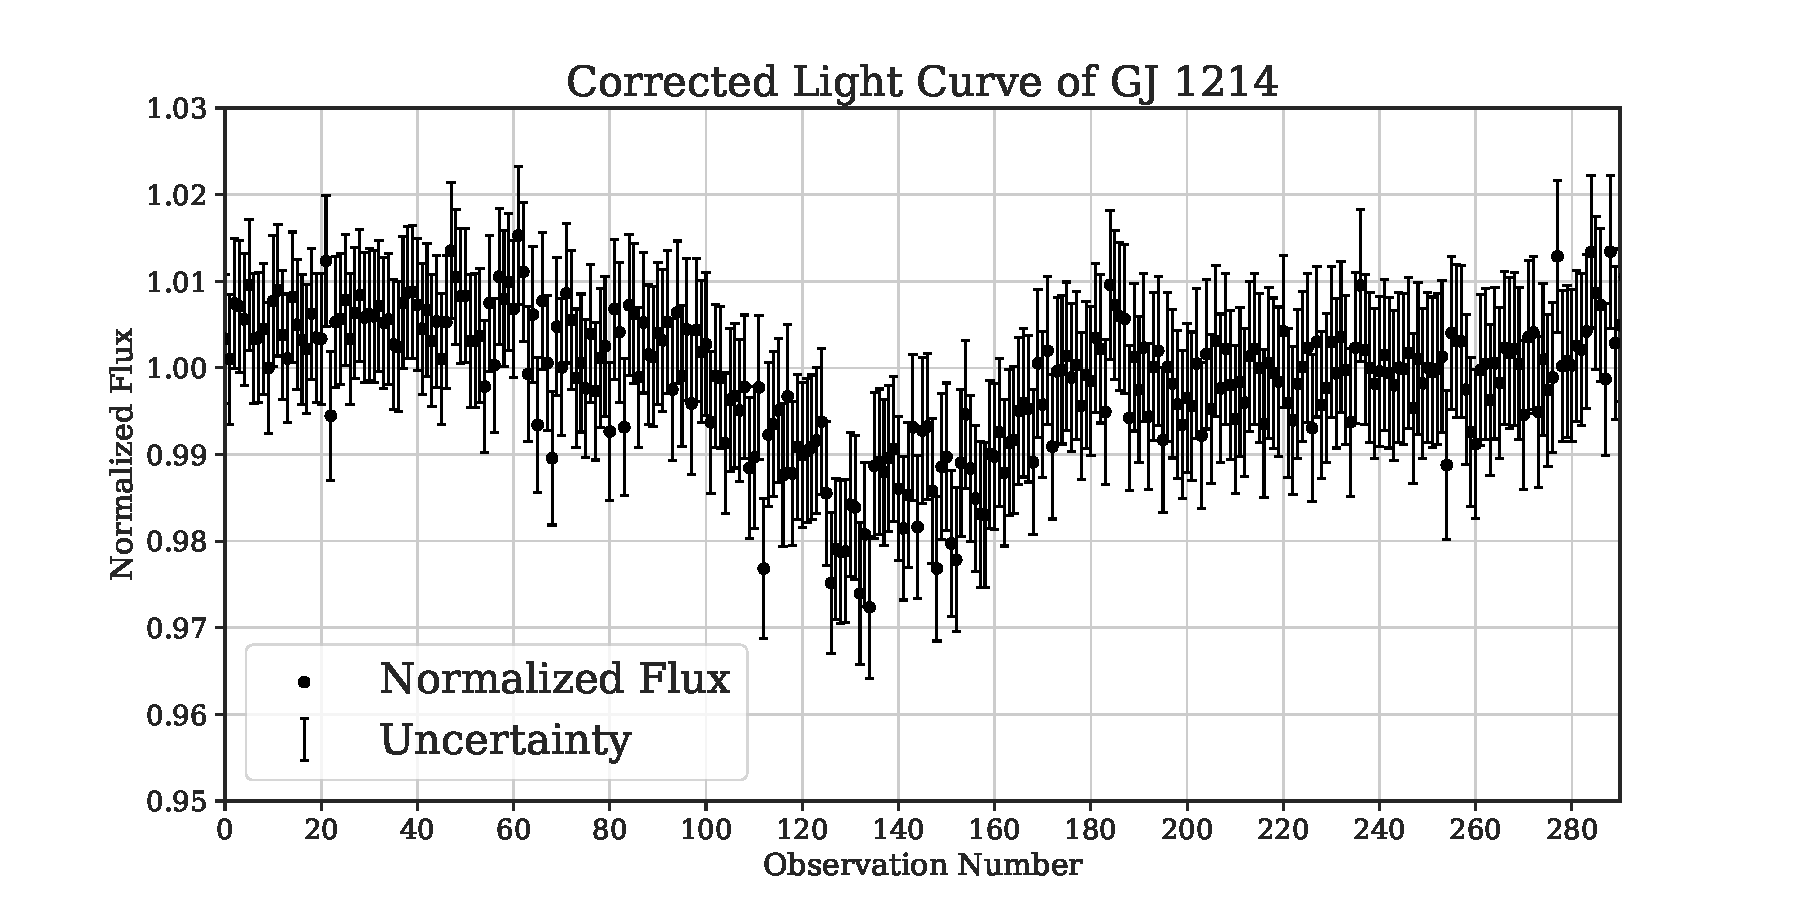
\includegraphics[width=1\textwidth]{plt/corrected_light_curve.pdf}
    \caption{The reduced light curve of GJ 1214 generated using the weighted mean reference curve, plotted with respect to observation number.}
    \label{fig:reduced_curve}
\end{figure}

\section{Data Analysis \& Modeling}
\subsection{A Rough Estimate of GJ 1214b's Parameters}
Using only a visual estimate, parameter's of GJ 1214b are already able to be estimated. By calculating the median flux inside and outside 
the time of transit, the depth of the transit can be estimated. A visualization of how this is done is shown in Figure \ref{fig:depth}.

\begin{figure}[H]
    \centering
    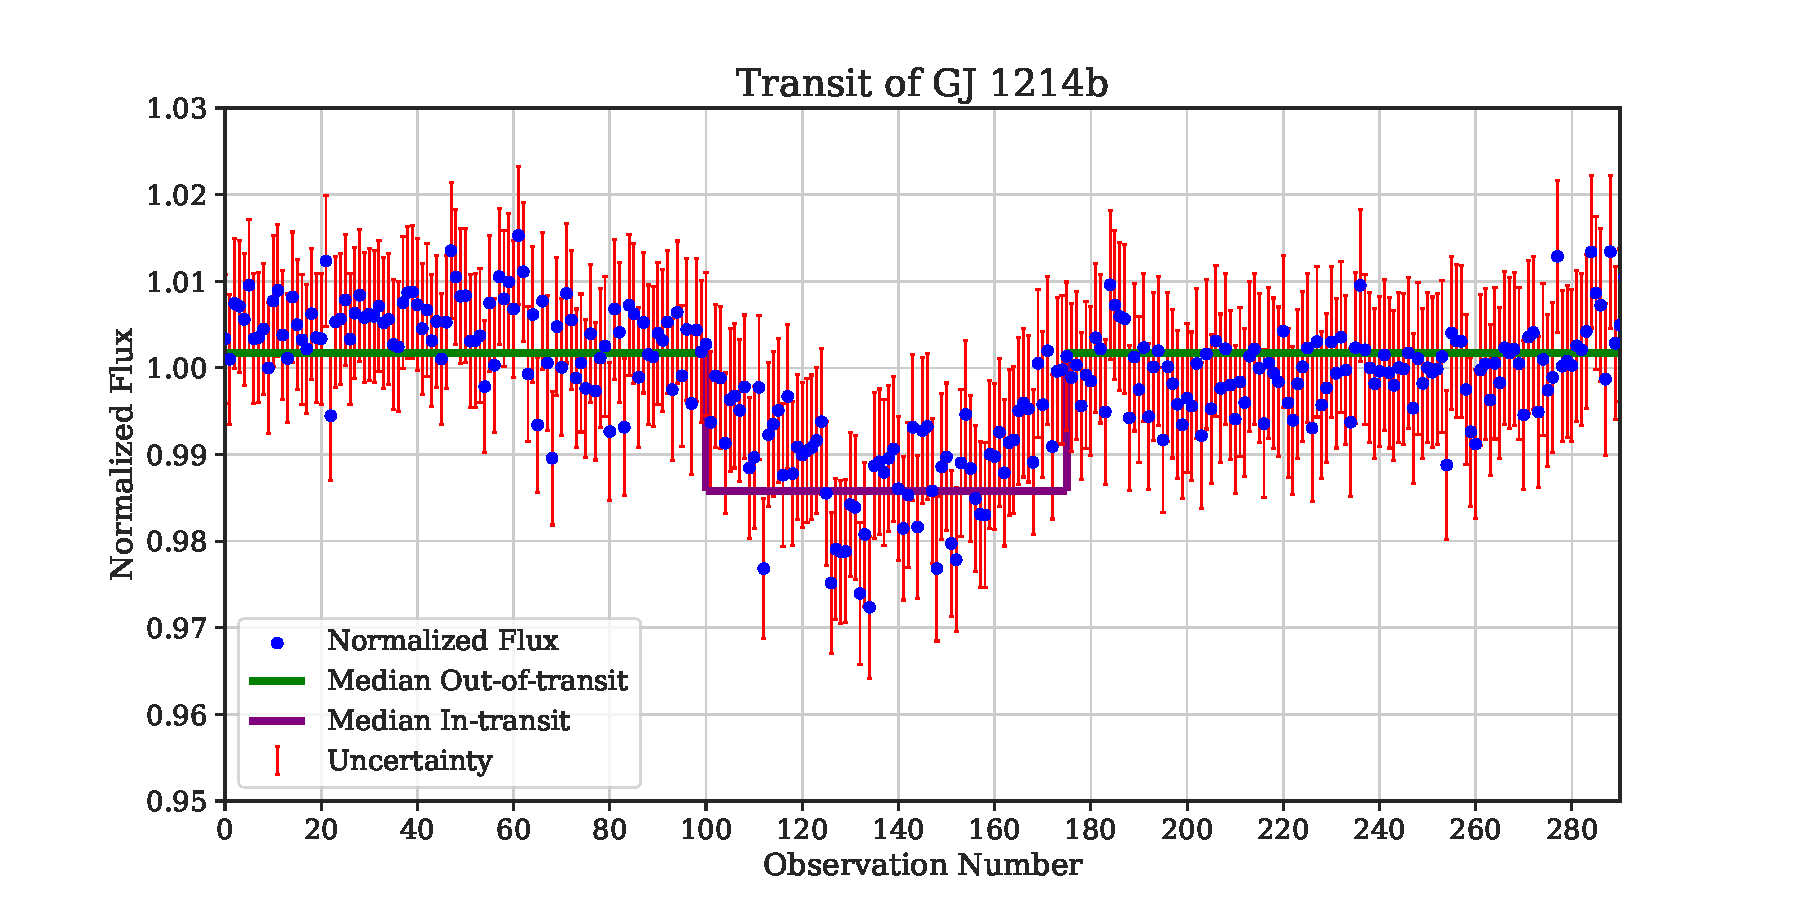
\includegraphics[width=1\textwidth]{plt/transit_estimate.pdf}
    \caption{A visual estimation of the transit of GJ 1214b.}
    \label{fig:depth}
\end{figure}

Since we only have data from one transit, the period is unable to be easily estimated. For this value, the period from The Extrasolar Planets Encyclopaedia\cite*{exo_encyclopedia}
is taken, which is $\approx 1.58$ days. The masses of GJ 1214 and GJ 1214b are also taken from the same source, which are $M_{s} \approx 0.15 M_{\odot}$, and $M_{p} \approx 8.17 M_{\oplus}$. The semi-major axis of GJ 1214b's orbit can then be calculated 
using Kepler's third law:

\begin{gather}
    a = \left(\frac{P^2GM}{4\pi^2}\right)^{1/3} \approx 3R_{\odot}
\end{gather}

With this information, we are able to find the radius and density of GJ 1214b using the light curve. The difference in the 
in-transit and out-of-transit regions is a $1.59 \%$ reduction in flux. We can use the proportionality between 
$\delta F$ and the planet-star radius ratio to determine the radius of GJ 1214b, from this we can find GJ 1214b's density as well: 

\begin{gather}
    \delta F = (\frac{R_p}{R{\star}})^2 \longrightarrow R_p = R_{\star}\sqrt{\delta F} \approx 0.027R_{\odot} \approx 2.95R_{\oplus} \\
    \rho \approx \frac{3 \times 8.17M_{\oplus}}{4\pi (2.95R_{\oplus})^3} \approx 1.75 \frac{g}{cm^3}
\end{gather}

From the light curve, it is also observed that the total time in transit is approximately 54 minutes. 

\subsection{Limb Darkening}
To estimate GJ 1214b's parameters more accurately, a model that includes the effects of limb darkening is fit to the light curve using SciPy's linear least-
squares fitting tool, \verb|curve_fit()|. The code was developed by Mandel \& Agol (2002)\cite*{limb2}, and Carter \& Yee (2008)\cite*{limb1}. To perform the fitting, four 
parameters are required as inputs to the model. These are the time dependent function $z(t)$ that is referenced in the two papers, the planet to star ratio $\frac{R_p}{R_{\star}}$, as
well as the limb darkening coefficients $c_1$ and $c_2$. By using the effective surface temperature and surface gravity of GJ 1214, a starting estimation of the limb darkening coefficients 
are found using the table provided by Claret (2004) \cite*{claret}. These initial guesses are not perfect, and are improved through the least-squares fit. The results of the fitting are shown in \ref{fig:limb_fit}, including
the final estimated values of the parameters and their uncertainties.

\begin{figure}[H]
    \centering
    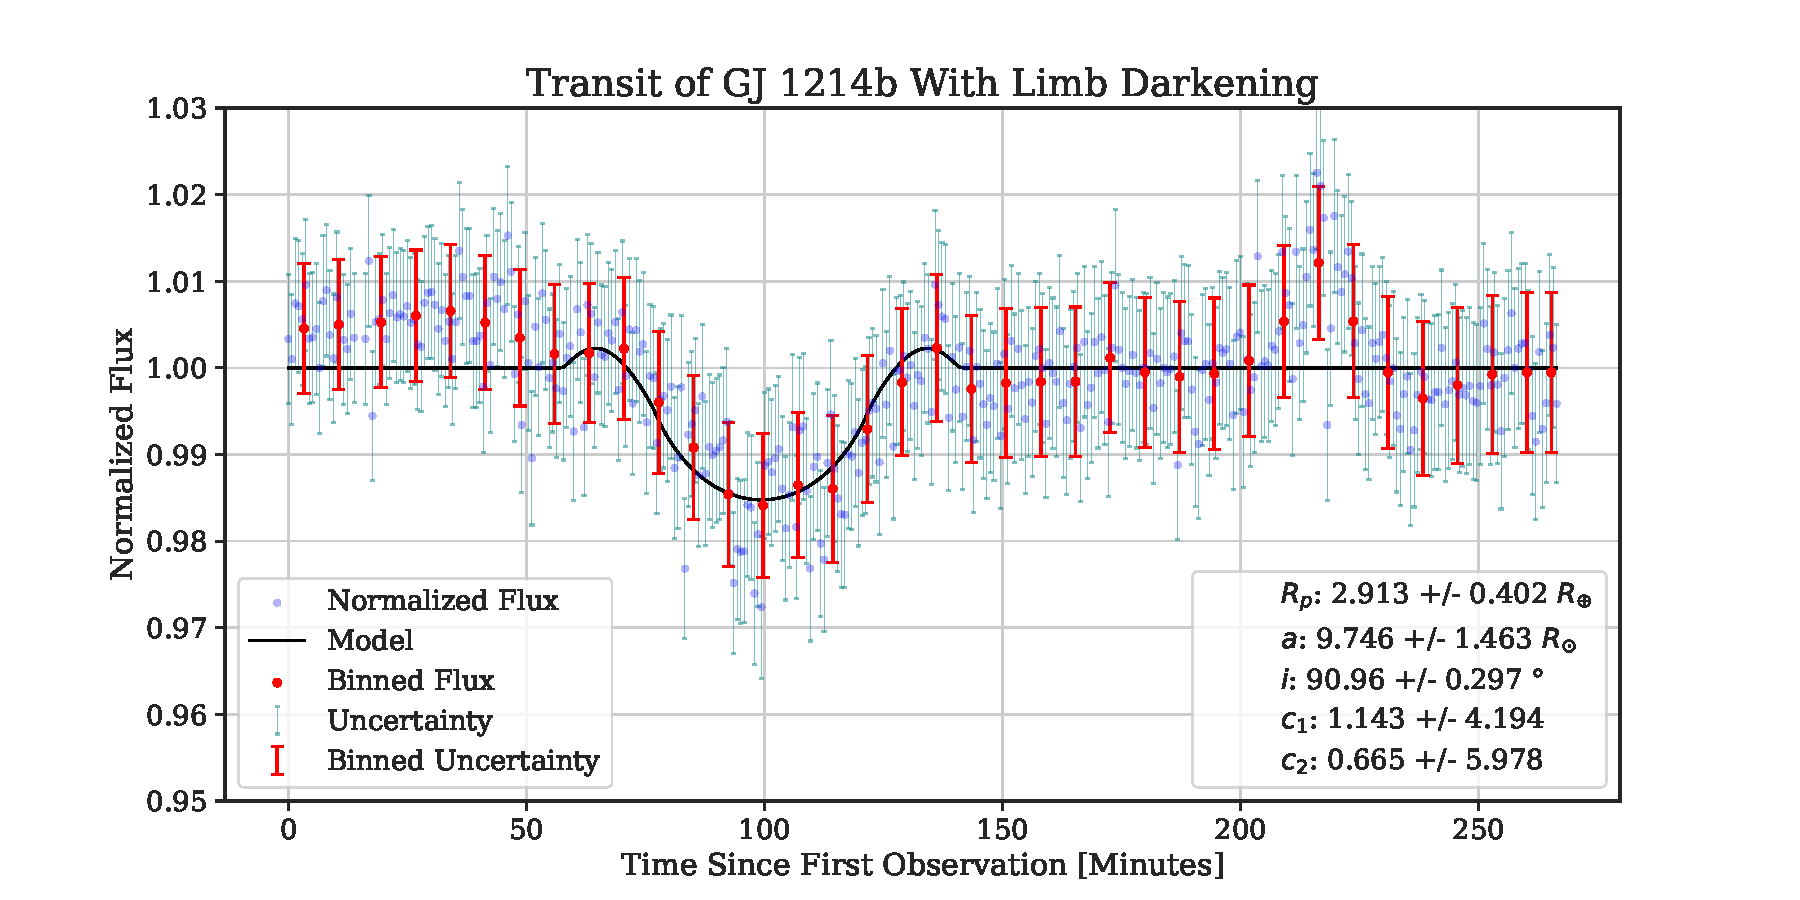
\includegraphics[width=1\textwidth]{plt/limb.pdf}
    \caption{The results of the linear least-squares fitting with limb darkening. The parameters of the fit include their final respective uncertainties.}
    \label{fig:limb_fit}
\end{figure}

\section{Discussion \& Error Analysis}
There are a number of sources of error that could contribute to the final results. The first of these is the centroid placement of the reference and target stars. This error is very hard to quantify, since the centroids were 
technically only calculated for a single image. This means that the error in this measurement is most likely dominated by the error in the translation of the centroids between images. This error was found to be $\approx 1-2$ pixels, 
and is deemed to be negligible in comparison to the other sources of error. The second source of error is the error in the flux measurements of the reference stars. This error turned out to be quite significant, especially after performing differential photometry on GJ 1214 and normalizing them. 
The flux uncertainties were also suspiciously uniform and somewhat larger than expected, which makes me think there may have been some kind of error in their calculations, despite double-checking my formula and code to make sure everything
was working properly. 

The third source of error, and most significant, is the error in the limb darkening fitting model. I had great difficulties getting the limb darkening model to fit my data properly, and you may notice that the shape of the fitted curve
does not match the shape of the data very well, and is not flat at the edges of the transit like a typical exoplanet transit plot should be. I attempted to constrain the parameters in different ways, and I found that when I constrained the fitting in such a way that the edges were flat, my final uncertainties were of
many magnitudes higher, of the order of hundreds of earths for the planet's radius. For this reason, I decided to leave the fitting in its current state, as most of the values are still pretty close to the ones I found in scientific papers. The only value that is quite far off 
is the semi-major axis, which I think may stem from an issue with the way I measured my fluxes. I noticed that the fluxes on each side of the transit are not even with each other, with the fluxes prior to the transit being higher than on the right. This could perhaps be fixed by using 
more reference stars for the differential photometry, as I could not use as many as I wanted to due to performance issues with my code and the computer I was using.   

\newpage

\printbibliography

\newpage

\begin{appendices}
\section{Python Code}
\subsection{Image Sorting \& Data Reduciton}
\begin{scriptsize}
\begin{verbatim}
from fileinput import filename
filenames = np.loadtxt('Lab5_ACAM_DATA/filelist', dtype=str, usecols=0)
flats = []
flats_hdu = []
biases = []
biases_hdu = []
science = []
science_hdu = []
for f in filenames:
    file = fits.open(r'Lab5_ACAM_DATA/' + f)
    header = file[0].header
    if header['OBSTYPE'] == 'FLAT':
        # print("-------")
        # print("File Name: ", f)
        # print("Image Type: ", header['OBSTYPE'])
        # print("Image Dimensions: ", file[1].data.shape)
        flats.append(file[1].data)
        flats_hdu.append(file[0].header)
    elif header['OBSTYPE'] == 'BIAS':
        if file[1].shape == (2071, 2148):
            # print("-------")
            # print("File Name: ", f)
            # print("Image Type: ", header['OBSTYPE'])
            # print("Instrument: ", header['INSTRUME'])
            # print("Exposure Time: ", header['EXPTIME'])
            # print("Image Dimensions: ", file[1].data.shape)
            biases.append(file[1].data)
            biases_hdu.append(file[0].header)
    elif header['OBSTYPE'] == 'TARGET':
        # print("-------")
        # print("File Name: ", f)
        # print("Image Type: ", header['OBSTYPE'])
        # print("Instrument: ", header['INSTRUME'])
        # print("Exposure Time: ", header['EXPTIME'])
        # print("Image Dimensions: ", file[1].data.shape)
        science.append(file[1].data)
        science_hdu.append(file[0].header)
        
science_np = np.array(science)
flats_np = np.array(flats)
biases_np = np.array(biases)

# Create mask for region outside vignette
threshold = 13000
mask = np.where(flats_np[0] > threshold, True, False)

# Normalize by exp time
for i in range(len(flats)):
    flats_np[i] = flats_np[i] * mask
    flats_np[i] = flats_np[i] / flats_hdu[i]['EXPTIME']
for i in range(len(science)):
    science_np[i] = science_np[i] * mask
    science_np[i] = science_np[i] / science_hdu[i]['EXPTIME']
    
# Median bias and flats
median_bias = np.median(biases_np*mask, axis=0)
median_flat = np.median(flats_np, axis=0)
median_flat = median_flat / np.median(median_flat)
median_bias = median_bias / np.median(median_bias)

for i in range(len(science_np)):
    science_np[i] = science_np[i] - (median_bias)
    science_np[i] = science_np[i] / median_flat
\end{verbatim}
\end{scriptsize}


\subsection{Function for Centroid \& Gaussian Fitting}
\begin{scriptsize}
\begin{verbatim}
from scipy.optimize import curve_fit

def star_gaussian(stars, image, size=10, filter=False): 
    uncertainties = []   
    centroids_x_coords = []
    centroids_y_coords = []
    initial_cen_x = []
    initial_cen_y = []
    app_radiuses = []

    failed_fittings = 0
    size = size
    
    # 2d gaussian
    def gauss(xy, a, x0, y0, sigma_x, sigma_y, c):
        x, y = xy
        g = a*np.exp(-(x-x0)**2/(2*sigma_x**2) - (y-y0)**2/(2*sigma_y**2)) + c
        return g.ravel()

    for i in range(len(stars[0])):
        box = image[int(stars[1][i])-size:int(stars[1][i])+size, int(stars[0][i])-size:int(stars[0][i])+size]
        
        # Create coordinate matrices and flatten them for fitting
        xx, yy = np.meshgrid(np.arange(box.shape[1]), np.arange(box.shape[0])) 
        xx_flat = xx.ravel()
        yy_flat = yy.ravel()

        # Use centroid equation for initial guess
        x = np.sum(xx * box) / np.sum(box) 
        y = np.sum(yy * box) / np.sum(box) 
        # Fit Gaussian
        if len(yy_flat) != 0:            
            try:
                initial_guess = (250,x,y,size/2,size/2,0)
                popt, pcov = curve_fit(gauss, (xx_flat, yy_flat), box.ravel(), p0=initial_guess, nan_policy='omit')
                if filter:
                    if np.max(np.sqrt(np.diag(pcov))) < 0.0125:
                            
                        # get new centroid
                        centroid_x, centroid_y = popt[1], popt[2]
                        
                        # put the coords back in the original context of the image
                        x = stars[0][i] - size + x
                        y = stars[1][i] - size + y
                        
                        centroid_x = stars[0][i] - size + centroid_x
                        centroid_y = stars[1][i] - size + centroid_y
                        
                        # print(f"Initial Coordinate: {stars[0][i]}, {stars[1][i]}")
                        # print(f"Inital Centroid: {x}, {y}")
                        # print(f"Gaussian Centroid: {centroid_x}, {centroid_y}")
                        
                        # add centroids to list of coords
                        initial_cen_x.append(x)
                        initial_cen_y.append(y)
                        centroids_x_coords.append(centroid_x)
                        centroids_y_coords.append(centroid_y)
                        uncertainties.append(np.max(np.sqrt(np.diag(pcov))))
                else:
                    centroid_x, centroid_y = popt[1], popt[2]
                    # put the coords back in the original context of the image
                    x = stars[0][i] - size + x
                    y = stars[1][i] - size + y
                    
                    centroid_x = stars[0][i] - size + centroid_x
                    centroid_y = stars[1][i] - size + centroid_y
                    
                    app_radiuses.append(max(3*np.abs(popt[4]), 3*np.abs(popt[3]))) # Use maximum of 3-sigma in x or y                     
                    
                    # print(f"Initial Coordinate: {stars[0][i]}, {stars[1][i]}")
                    # print(f"Inital Centroid: {x}, {y}")
                    # print(f"Gaussian Centroid: {centroid_x}, {centroid_y}")
                    
                    # add centroids to list of coords
                    initial_cen_x.append(x)
                    initial_cen_y.append(y)
                    centroids_x_coords.append(centroid_x)
                    centroids_y_coords.append(centroid_y)
                    uncertainties.append(np.max(np.sqrt(np.diag(pcov))))
                
            except RuntimeError:
                failed_fittings += 1
    # print(f"Fit {len(centroids_x_coords)} stars")
    # print(f"Couldn't fit {failed_fittings} stars")
    #print("Radius: ", app_radius)
    return centroids_x_coords, centroids_y_coords, initial_cen_x, initial_cen_y, uncertainties, app_radiuses
\end{verbatim}
\end{scriptsize}

\subsection{Image Displacement Tracking}
\begin{scriptsize}
\begin{verbatim}
# Track star throughout the observations to approximate global displacement
stars_x = [790]
stars_y = [710]
box=40

centroid_x = []
centroid_y = []
approx_x = []
approx_y = []
uncertainties = []

for i in range(len(science_np)):
    x, y, cen_x, cen_y, uncertainties, _ = star_gaussian([stars_x,stars_y], science_np[i], size=box, filter=False) 
    centroid_x.append(x)
    centroid_y.append(y)
    approx_x.append(cen_x)
    approx_y.append(cen_y)
    uncertainties.append(uncertainties)
    if (len(x) == 0) or (len(y) == 0):
        print(f"Failed to find star in image {i}")

x_motion = np.array([centroid_x[i][0] - centroid_x[0][0] for i in range(len(centroid_x))])
y_motion = np.array([centroid_y[i][0] - centroid_y[0][0] for i in range(len(centroid_y))])
magnitude = np.sqrt(x_motion**2 + y_motion**2)
\end{verbatim}
\end{scriptsize}

\subsection{Star Finding Using Binary Mask}
\begin{scriptsize}
\begin{verbatim}
threshold = 85
stars_x = []
stars_y = []
aperture_radius = []

# Find parts of img where intensity > threshold
binary_img = np.where(science_np[0] > threshold, 1, 0)

# Assign each star region a different integer
star_labels, num_stars = label(binary_img)
print(f"Found {num_stars} stars")

# Loop through each region and pick a single point to feed the centroider.
for i in range(1,num_stars+1):
    region_coords = np.where(star_labels == i)
    # Use middle point in each region
    middle_x = np.mean(region_coords[0]).astype(int)
    middle_y = np.mean(region_coords[1]).astype(int) 
    stars_x.append(middle_y)
    stars_y.append(middle_x)
    
size=15
centroid_x, centroid_y, init_x, init_y, position_uncertainties, rad = star_gaussian([stars_x, stars_y], science_np[0], size=size)
centroid_catalog = pd.DataFrame({'centroid_x': centroid_x, 'centroid_y': centroid_y, 'aperture_radius': rad})

# Save centroids
centroid_catalog.to_csv('centroid_catalog.csv')

### For removing bad stars
# centroid_catalog = centroid_catalog.drop([0,5,17,19])
# centroid_catalog = centroid_catalog.reset_index(drop=True)

# ## Check the centroids individually
# vmin, vmax = ZScaleInterval().get_limits(science_np[0])
# for i in range(len(centroid_catalog)):
#     plt.title(f"Reference {i}")
#     plt.imshow(science_np[0], cmap='cma:lacerta', vmin=vmin,vmax=vmax)
#     plt.scatter(centroid_catalog['centroid_x'], centroid_catalog['centroid_y'], c='r', s=40, label="Gaussian Centroid", marker='x')
#     plt.scatter(init_x,init_y, c='b', s=40, label="Traditional Centroid", marker='x')
#     plt.xlim(centroid_catalog['centroid_x'][i]-size, centroid_catalog['centroid_x'][i]+size)
#     plt.ylim(centroid_catalog['centroid_y'][i]-size, centroid_catalog['centroid_y'][i]+size)
#     plt.legend()
#     plt.show()

######## TARGET STAR ########
target_approx_x = 1419
target_approx_y = 817
target_centroid_x, target_centroid_y, _, _, _, target_rad = star_gaussian([np.array([target_approx_x]), np.array([target_approx_y])], science_np[0], size=8, filter=False)
size = 650

# for i in range(len(science_np)):
#     plt.imshow(science_np[i], cmap='cma:lacerta', vmin=vmin,vmax=vmax)
#     xcenter = target_centroid_x[0] + x_motion[i]
#     ycenter = target_centroid_y[0] + y_motion[i]
#     plt.scatter(xcenter,ycenter, c='r', s=2)
#     plt.xlim(xcenter-size, xcenter+size)
#     plt.ylim(ycenter-size, ycenter+size)
#     plt.show()
\end{verbatim}
\end{scriptsize}


\subsection{Aperture Photometry}
\begin{scriptsize}
\begin{verbatim}
gain = 4 # e/DN
def aperture_photometry(image, x, y, xcenter, ycenter, app_radius, inner_radius, outer_radius, plot=False):
    def annulus():
        r_squared = (x - xcenter)**2 + (y - ycenter)**2
        mask = (r_squared <= outer_radius**2) & (r_squared >= inner_radius**2)
        annulus_sum = np.sum(image * mask)
        num_pixels = np.sum(mask)
        level_per_pixel = annulus_sum / num_pixels
        
        # Uncertainty
        sigma_bg = np.std(image*mask)

        if plot:
            plt.xlim(xcenter-20,xcenter+20)
            plt.ylim(ycenter-20,ycenter+20)
            vmin,vmax = ZScaleInterval().get_limits(image)
            plt.imshow(image, vmin=-vmin, vmax = vmax, origin='lower', cmap='cma:lacerta')
            plt.imshow(mask, origin='lower', cmap='gray', alpha=0.6)
            plt.savefig("plt/annulus.pdf")
            plt.show()
        return level_per_pixel, sigma_bg
    
    def aperture():
        mask = ((x - xcenter)**2 + (y - ycenter)**2) <= app_radius**2
        aperture_sum = np.sum(image * mask)
        if plot:
            plt.xlim(xcenter-20,xcenter+20)
            plt.ylim(ycenter-20,ycenter+20)
            vmin,vmax = ZScaleInterval().get_limits(image)
            plt.imshow(image, vmin=vmin, vmax = vmax, origin='lower', cmap='cma:lacerta')
            plt.imshow(mask, origin='lower', cmap='inferno', alpha=0.6)
            plt.savefig("plt/aperture.pdf")
        plt.show()
        return aperture_sum, mask
    
    def uncertainty(flux,sigma_bg,num_aperture,num_annulus):
        return np.sqrt(flux/gain + num_aperture*(1+(np.pi*num_aperture)/(2*num_annulus)*sigma_bg**2))

    flux = aperture()[0] - annulus()[0]
    error = uncertainty(flux, annulus()[1], np.sum(aperture()[1]), np.sum(annulus()[1]))
    return flux, error

def process_observation(i, j=0):
    xcenter = centroid_catalog['centroid_x'][j] + x_motion[i]
    ycenter = centroid_catalog['centroid_y'][j] + y_motion[i]
    inner_radius = centroid_catalog['aperture_radius'][j] + 6
    outer_radius = centroid_catalog['aperture_radius'][j] + 14
    app_radius = centroid_catalog['aperture_radius'][j]
    flux, flux_uncertainty = aperture_photometry(science_np[i], x, y, xcenter, ycenter, app_radius, 
                                            inner_radius, outer_radius, plot=False)
    return pd.DataFrame({'Observation': [i], 'star_number': [j], 'centroid_x': [xcenter], 
                            'centroid_y': [ycenter], 'flux': [flux], 'uncertainty': [flux_uncertainty]})

# #Uncomment for fresh data
ysize, xsize = science_np[0].shape
y, x = np.mgrid[:ysize, :xsize]
# results = []
# for i in range(len(science_np)):
#     print(f"Observation {i} / {len(science_np)-1}")
#     print("---")
#     for j in range(len(centroid_catalog)):
#         #print("Star ", j)
#         obs = process_observation(i, j)
#         results.append(obs)
# full_df = pd.concat(results)
# full_df.to_csv('flux_database.csv', index=False)

# ### TARGET FLUX #####
# results = []
# for i in range(len(science_np)):
#     xcenter = target_centroid_x[0] + x_motion[i]
#     ycenter = target_centroid_y[0] + y_motion[i]
#     inner_radius = target_rad[0] + 10
#     outer_radius = target_rad[0] + 20
#     flux, flux_uncertainty = aperture_photometry(science_np[i], x, y, xcenter, ycenter, target_rad[0], 
#                                             inner_radius, outer_radius,plot=False)
#     print(f"Observation {i} - Flux: {flux} +/- {flux_uncertainty}")
#     obs = pd.DataFrame({'Observation': [i], 'centroid_x': [xcenter], 
#                          'centroid_y': [ycenter], 'flux': [flux], 'uncertainty': [flux_uncertainty]})
#     results.append(obs)
#target_df = pd.concat(results)
#target_df.to_csv('target_flux_database.csv', index=False)

flux_database = pd.read_csv('flux_database.csv')


############ Remove star_number 8 (Transit Star)
flux_database = flux_database[flux_database['star_number'] != 9]

# Compute the median flux of each star
medians = flux_database.groupby('star_number')['flux'].median()

# Divide the fluxes by the median flux of their star
flux_database['norm_flux'] = flux_database.groupby('star_number')['flux'].transform(lambda x: x / medians[x.name])

# Also scale the errors by median flux
flux_database['norm_uncertainty'] = flux_database.groupby('star_number')['uncertainty'].transform(lambda x: x / medians[x.name])

######### Remove any wack curves
flux_database = flux_database[~flux_database['star_number'].isin([7,25,19,28,27,30])]
flux_database = flux_database[~flux_database['star_number'].isin([0,3])] 
#flux_database = flux_database[~flux_database['star_number'].isin([13,14])] 
flux_database = flux_database.reset_index(drop=True)
\end{verbatim}    
\end{scriptsize}

\subsection{Generate and Apply Reference Light Curves}
\begin{scriptsize}
\begin{verbatim}
# Median Reference Curve
median_reference = flux_database.groupby('Observation')['norm_flux'].median()
flux_database['median_reference'] = flux_database['Observation'].map(median_reference)

# Weighted Mean Reference Curve
fig = plt.figure(figsize=(12,6))
weights = 1./flux_database['norm_uncertainty']**2
weighted_mean_reference = flux_database.groupby('Observation').apply(lambda x: np.average(x['norm_flux'], weights=weights[x.index]))
weighted_mean_uncertainty = flux_database.groupby('Observation').apply(lambda x: 1/np.sqrt(np.sum(weights[x.index])))
flux_database['weighted_mean_reference'] = flux_database['Observation'].map(weighted_mean_reference)

# Median Normalize Target
target_flux = pd.read_csv('target_flux_database.csv')
norm_target_flux = target_flux['flux']/np.median(target_flux['flux'])
norm_target_uncertainty = target_flux['uncertainty']/np.median(target_flux['flux'])

# Get the times from the headers
dates = [hdu['DATE-OBS'] for hdu in science_hdu]
times = [hdu['UTSTART'] for hdu in science_hdu]
datetime_strings = [f"{dates[i]} {times[i]}" for i in range(len(dates))]
datetimes = [datetime.strptime(s, "%Y-%m-%d %H:%M:%S.%f") for s in datetime_strings]
time_since_first_obs = [(dt - datetimes[0]).total_seconds() for dt in datetimes] # seconds
min_since_first_obs = [t/60 for t in time_since_first_obs] # minutes

# Apply reference curves to target star
# Median Reference
target_flux['corrected_flux_median'] = norm_target_flux / target_flux['Observation'].map(median_reference)
target_flux['corrected_flux_median'] = target_flux['corrected_flux_median'] / np.median(target_flux['corrected_flux_median'])

# Mean Reference
target_flux['corrected_flux_weighted'] = norm_target_flux / target_flux['Observation'].map(weighted_mean_reference)
target_flux['corrected_flux_weighted'] = target_flux['corrected_flux_weighted'] / np.median(target_flux['corrected_flux_weighted'])
target_flux['corrected_flux_mean_uncertainty'] = np.sqrt(norm_target_uncertainty**2 + weighted_mean_uncertainty**2)

out_of_transit = target_flux[(target_flux['Observation'] < 100) | (target_flux['Observation'] > 180)]
median_out = np.median(out_of_transit['corrected_flux_weighted'])

in_transit = target_flux[(target_flux['Observation'] > 120) & (target_flux['Observation'] < 150)]
median_in = np.median(in_transit['corrected_flux_weighted'])
\end{verbatim}
\end{scriptsize}

\subsection{Estimating GJ 1214b's Parameters Using Flat-Top Model}
\begin{scriptsize}
\begin{verbatim}


transit_depth = abs(median_in - median_out)  # values are already normalized
print(f"Change in flux during transit: {transit_depth*100:.2f}%")

star_radius = 0.216  # R sun
#star_radius_au = star_radius / 215  # AU
star_radius_au = 0.0010045009

# take square root of depth to calculate planet-star radius ratio
radius_ratio = np.sqrt(transit_depth) 

# multiply by star_radius to get estimated planet radius
estimated_radius = radius_ratio * star_radius
estimated_radius_au = radius_ratio * star_radius_au

print("Start of Transit: ", min_since_first_obs[100])
print("End of Transit: ", min_since_first_obs[175])
print("Duration of Transit: ", min_since_first_obs[175] - min_since_first_obs[100], "minutes")
print(f"Planet Star Ratio (R_p/R_s): {radius_ratio}")
print(f"Estimated Radius (Solar Radii): {estimated_radius}")
print(f"Estimated Radius (Jupiter Radii): {estimated_radius*9.95551486890475}")

\end{verbatim}
\end{scriptsize}


\subsection{Limb Darkening}
\begin{scriptsize}
\begin{verbatim}
from occultquad import occultquad

# Binned data
def bin_data(data, bin_size):
    binned_data = []
    for i in range(0, len(data), bin_size):
        binned_data.append(np.mean(data[i:i+bin_size]))
    return binned_data
bin_size = 10
binned_data = bin_data(target_flux['corrected_flux_weighted'], bin_size)
binned_positions = bin_data(min_since_first_obs, bin_size)
binned_uncertainty = bin_data(target_flux['corrected_flux_mean_uncertainty'], bin_size)
binned_data_np = np.array(binned_data)

# (Claret, 2004 Vizier), and exoplanet enc. 
c1 = .4065
c2 = .3753	
a = 0.01411  # AU
radius_guess = 0.0001169073322 # AU
orbital_period_minutes = 2275.78247568 # minutes

i=np.deg2rad(90)
time = min_since_first_obs[50:200]
# Find center of transit 
t_c_est = min_since_first_obs[np.where(target_flux['corrected_flux_weighted'] == np.min(target_flux['corrected_flux_weighted']))[0][0]]

def lc_model(time,r_p,a,i,c1,c2):
    def z(t):
        omega = 1 / orbital_period_minutes # rad/min
        return (a/star_radius_au)*(np.sqrt((np.sin(omega*t))**2 + (np.cos(i)*np.cos(omega*t))**2))

    curve_times = np.array(time) - t_c_est
    z_est = z(curve_times)
    radius_ratio = r_p / star_radius_au
    curve = occultquad(z_est,c1,c2,radius_ratio)[0]
    return curve
    

lower_bounds = [radius_guess - 0.01, a - 0.15,  i - .1, c1 - .4065, c2 - .3753]
upper_bounds = [radius_guess + 0.01, a + 0.15,  i + .1, c1 + .73658, c2 + 1]

popt, pcov = curve_fit(lc_model, time, target_flux['corrected_flux_weighted'][50:200], p0=[radius_guess,a,i,c1,c2], bounds=(lower_bounds, upper_bounds))
fit_error = np.array([np.sqrt(pcov[i,i]) for i in range(pcov.shape[0])])

print(f"Radius: {popt[0]*23450} +/- {fit_error[0]*23450} Earth Radii")
print(f"Semi-Major Axis: {popt[1]*215} +/- {fit_error[1]*215} Solar Radii")
print(f"Inclination: {np.rad2deg(popt[2])} +/- {np.rad2deg(fit_error[2])} Degrees")
print(f"Limb Darkening c1: {popt[3]} +/- {fit_error[3]}")
print(f"Limb Darkening c2: {popt[4]} +/- {fit_error[4]}")
\end{verbatim}
\end{scriptsize}


\end{appendices}

\end{document}